\documentclass[letterpaper,10pt]{article}

\usepackage{titling}
\usepackage{listings}
\usepackage{url}
\usepackage{setspace}
\usepackage{subfig}
\usepackage{sectsty}
\usepackage{pdfpages}
\usepackage{colortbl}
\usepackage{multirow}
\usepackage{multicol}
\usepackage{relsize}
\usepackage{amsmath}
\usepackage{wasysym}
\usepackage{fancyvrb}
\usepackage{amssymb}
\usepackage{ifsym}
\usepackage{amsmath,amssymb,amsthm,graphicx,xspace}
\usepackage[titlenotnumbered,noend,noline]{algorithm2e}
\usepackage[compact]{titlesec}
\usepackage{XCharter}
\usepackage[T1]{fontenc}
\usepackage{tikz}
\usetikzlibrary{arrows,automata,shapes,trees,matrix,chains,scopes,positioning,calc}
\tikzstyle{block} = [rectangle, draw, fill=blue!20, 
    text width=2.5em, text centered, rounded corners, minimum height=2em]
\tikzstyle{bw} = [rectangle, draw, fill=blue!20, 
    text width=4em, text centered, rounded corners, minimum height=2em]

\definecolor{namerow}{cmyk}{.40,.40,.40,.40}
\definecolor{namecol}{cmyk}{.40,.40,.40,.40}

\let\LaTeXtitle\title
\renewcommand{\title}[1]{\LaTeXtitle{\textsf{#1}}}


\newcommand{\handout}[5]{
  \noindent
  \begin{center}
  \framebox{
    \vbox{
      \hbox to 5.78in { {\bf ECE356: Database Systems } \hfill #2 }
      \vspace{4mm}
      \hbox to 5.78in { {\Large \hfill #4  \hfill} }
      \vspace{2mm}
      \hbox to 5.78in { {\em #3 \hfill} }
    }
  }
  \end{center}
  \vspace*{4mm}
}

\newcommand{\lecture}[3]{\handout{#1}{#2}{#3}{Lecture #1}}
\newcommand{\tuple}[1]{\ensuremath{\left\langle #1 \right\rangle}\xspace}

\addtolength{\oddsidemargin}{-1.000in}
\addtolength{\evensidemargin}{-0.500in}
\addtolength{\textwidth}{2.0in}
\addtolength{\topmargin}{-1.000in}
\addtolength{\textheight}{1.75in}
\addtolength{\parskip}{\baselineskip}
\setlength{\parindent}{0in}
\renewcommand{\baselinestretch}{1.5}
\newcommand{\term}{Winter 2018}

\singlespace


\begin{document}

\lecture{ 28 --- Data Warehousing \& Mining }{\term}{Jeff Zarnett}

\section*{Data Warehousing \& Mining}

Databases, as you know, truly run the world. Think about a company like Amazon (let's restrict ourselves for the moment to their online store business). They have accumulated a huge amount of data about the purchases made. There needs to be a way to store this very large volume of data. That is what data \textit{warehousing} is about. The purchase history of Amazon users between the years 2010 and 2015 is perhaps not needed on a regular basis, but it is saved and stored. But why? Because it can be mined: it provides insights.

\textit{Data mining} is about extracting information from a large volume of stored data.  The more data we have, the better predictions we can make. Amazon may know that 60\% of the time, someone who buys product $x$ will soon buy product $y$ -- and then can suggest $y$ to you on the page when you have added $x$ to your cart.

Now you might think that data mining is just helpful: Amazon is guessing about products I want and if they guess right, they are helping me! Maybe? But the truth is, this sort of data mining can be downright... creepy. Consider this story by Charles Duhigg, in the New York Times about how Target (the retailer) used the data it has to make predictions about whether a woman is expecting a child soon: 

\begin{quote}
Target has a baby-shower registry, and Pole started there, observing how shopping habits changed as a woman approached her due date, which women on the registry had willingly disclosed. He ran test after test, analyzing the data, and before long some useful patterns emerged. Lotions, for example. Lots of people buy lotion, but one of Pole's colleagues noticed that women on the baby registry were buying larger quantities of unscented lotion around the beginning of their second trimester. Another analyst noted that sometime in the first 20 weeks, pregnant women loaded up on supplements like calcium, magnesium and zinc. Many shoppers purchase soap and cotton balls, but when someone suddenly starts buying lots of scent-free soap and extra-big bags of cotton balls, in addition to hand sanitizers and washcloths, it signals they could be getting close to their delivery date.

As Pole's computers crawled through the data, he was able to identify about 25 products that, when analyzed together, allowed him to assign each shopper a ``pregnancy prediction'' score. More important, he could also estimate her due date to within a small window, so Target could send coupons timed to very specific stages of her pregnancy.

...


About a year after Pole created his pregnancy-prediction model, a man walked into a Target outside Minneapolis and demanded to see the manager. He was clutching coupons that had been sent to his daughter, and he was angry, according to an employee who participated in the conversation.

``My daughter got this in the mail!'' he said. ``She's still in high school, and you're sending her coupons for baby clothes and cribs? Are you trying to encourage her to get pregnant?''

The manager didn't have any idea what the man was talking about. He looked at the mailer. Sure enough, it was addressed to the man's daughter and contained advertisements for maternity clothing, nursery furniture and pictures of smiling infants. The manager apologized and then called a few days later to apologize again.

On the phone, though, the father was somewhat abashed. ``I had a talk with my daughter,'' he said. ``It turns out there's been some activities in my house I haven't been completely aware of. She's due in August. I owe you an apology.''
\end{quote}
\hfill --Charles Duhigg~\cite{targetdata}

More generally, data warehousing is used to prepare large amounts of data for mining, and the purpose of the mining is to be used in what is called a \textit{decision support system}. These are used not only to guess super personal information about shoppers, but also to tell store managers what products they should have in stock in what month, tell factory managers what products they should manufacture, and even (dare I say it) tell admissions officers what applicants should be admitted to a university~\cite{dsc}.

We'll first focus on how the data is to be aggregated (warehousing) before we get into a bit more about mining. The Target story makes for a compelling hook, but we have to eat our vegetables before we may have dessert.

\subsection*{Warehousing}

It is virtually a certainty that in any large organization, the data will be spread across different databases or other sources. More than that, data can come from external sources: mailing lists from marketing organizations, credit scores from ratings agencies, legacy systems from purchased subsidiary companies, et cetera~\cite{dsc}. To make things work, we will need to aggregate all this data somehow. The destination is the data warehouse, which contains large amounts of data in a common schema. There, the data resides for the long term and can be available for mining.

Consider a quick diagram from~\cite{dsc} that overviews data warehouse architecture: 

\begin{center}
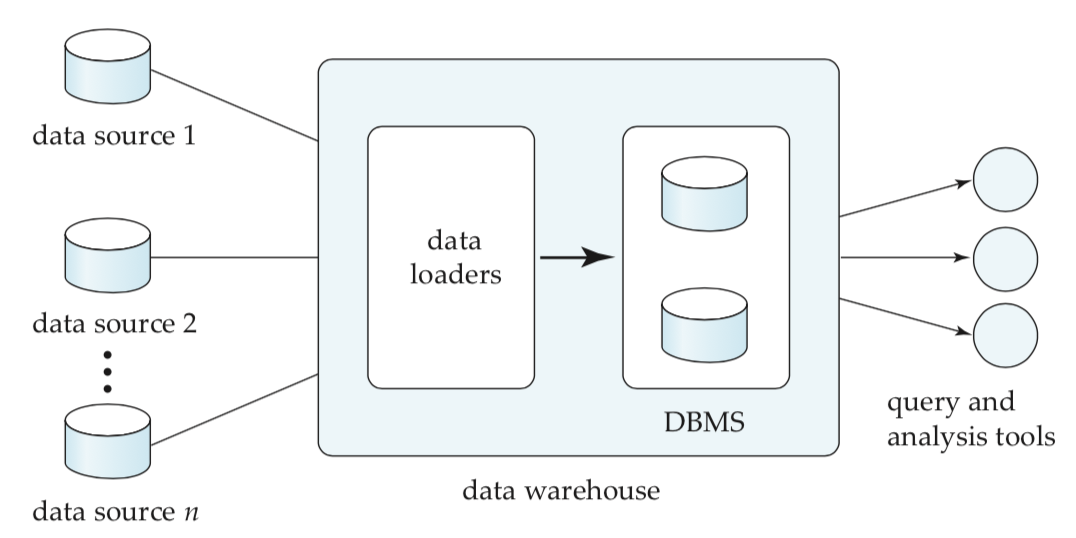
\includegraphics[width=0.75\textwidth]{images/warehouse}\\
Data warehousing architecture~\cite{dsc}
\end{center}

As we can see there are $n$ data sources that feed into the warehouse. Each data source is associated with a ``loader''; some sort of transformation routine that converts incoming data into the appropriate format for the warehouse's DBMS. Then the data is available for use in query and analysis tools.

The decision about when and how to gather data is important but perhaps boring. Data can be transferred from the original source to the warehouse periodically (e.g., every night), on demand (when a refresh is requested, automatically or manually), based on a certain volume of data (e.g., every $n$ transactions)... There are many many options. Whatever we do, data is likely to be at least slightly out of date: today's purchases, for example, might not be in warehouse yet because they are not yet completed and closed. That is fine; even though the data may be slightly out of date we can still make good decisions or predictions based on what we have.

The decision of what schema to use in the warehouse will obviously depend on what the query and analysis tools are for. Importing the data requires transformation and with good luck all that is needed is a straight 1-to-1 mapping where this field corresponds to that field and all is well. Where things become difficult is when data is not so clean and consistent.

There is therefore the process of \textit{data cleansing}: cleaning up minor inconsistencies in the data by correcting them~\cite{dsc}. As examples, names and addresses can be misspelled (especially if a name is uncommon or uses a less favoured spelling...) and so the same human may be represented by the names ``Megan'' and ``Meghan'' due to some entry error in one of the databases. We've already examined, to some degree, the idea of how we could repair such inconsistencies by examining the various probabilities of correctness of each value: if the name is ``Meghan'' in twelve places and ``Megan'' in one, we think it is likely the spelling with the ``h'' is correct.

You have probably already seen the idea of data cleansing on the small scale: if you have multiple contacts with the same name in your phone address book, it may suggest that you merge these contacts (if they are in fact the same person). This is de-duplication, that is, duplicate elimination. 

Interestingly, we might want to use column-oriented storage in the warehouse rather than the standard row-oriented storage. It is noted in~\cite{dsc} that there might be two advantages: (1) if we are fetching only a few attributes, we get exactly what we need rather than having to throw away parts of rows we don't need; and (2) storing things of the same type makes compression possible. But the drawback is that accessing a single row means multiple I/O operations. 

\subsection*{Mining}

With the data stored, now we want to use it. As we have already seen, in addition to statistical data, the data warehouse allows predictions or discovery of ``new'' information. There are three kinds of information we could discover~\cite{fds}:

\begin{itemize}
	\item \textbf{Association Rules}: One type of event is likely to take place at the same time as another: e.g., people who purchase a DSLR camera are likely to purchase a set of rechargeable batteries to go with it.
	\item \textbf{Sequential Patterns}: One event is likely to lead to another in the future: e.g., a person who buys a printer is likely to purchase a new toner cartridge within the next year.
	\item \textbf{Classification Trees}: Individuals (people) can be classified based on patterns of their behaviour: e.g., a person who purchases more than \$x in a given year is a ``top customer'' and should receive some preferential treatment.
\end{itemize}

\paragraph{Association.} We'll start off by looking at association. The example from~\cite{dsc} we will use has to do with credit scores. To sum up how this works, a credit score is a way of assessing the likelihood that a person borrowing money will repay the money. Credit scores are represented by three digit scores generally, but they are obviously more complex than that. The best way of predicting whether or not someone is likely to repay a loan is, of course, their previous behaviour. But for someone who doesn't have a credit history (e.g., a person who has just graduated university) we might try to use some association data to predict (1) whether we should lend this person money and (2) if so, at what interest rate.

Suppose then there are four categories for credit: bad, average, good, and excellent. Then we need to figure out what are the key elements that determine someone's repayment history. We have some amount of data on an individual: place of birth, educational attainment, age, gender, income, marital status, and many more items. Some of the information we have is  not relevant; some of it is. What we are looking for is a statistical correlation that says, for example, repayment of a loan is correlated with higher income. I'll assume you have a pretty good idea of how a statistical correlation is generated.

The data that we have is our \textit{training set}. The training set is used to produce the rules by finding the correlations. What we should actually do is use a subset of the data as the training set. Then we verify the predictive power of the rules we have developed by looking at the rest of the data to see if the predictions match reality.

Now, in theory we could use every piece of available data to make a prediction, but realistically we only care about those elements that have a correlation and predictive value. And to prevent things from getting out of hand, we might pick only a top few items, ranking them from strongest correlation to weakest. Using those we can then build a tree that will be used to classify the creditworthiness of people for whom we have no (or limited) data.

It's worth noting that sometimes data may point to certain correlations, but it would be unethical to use it. Discrimination based on elements like ethnicity, gender, religion, anything like that is unethical if not illegal in a given jurisdiction. We might have the data in our database, though, or be able to find it out. It is still not okay to use.

In the creditworthiness example, let us assume the data we have says the biggest predictor of loan repayment is degree attainment, and the next biggest is income. If we are looking only at the top two elements (or all others produce a correlation below a certain cutoff) then we could construct a tree that looks something like:
\begin{center}
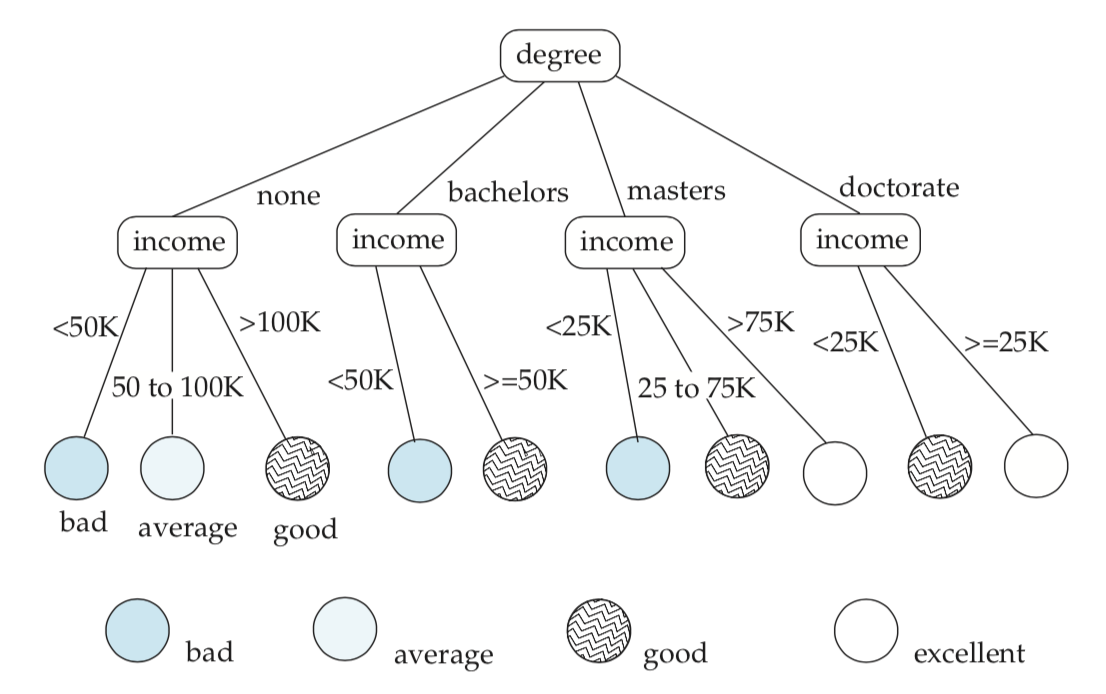
\includegraphics[width=0.75\textwidth]{images/classification-tree}\\
A classification tree for credit risks based on degree attainment and income~\cite{dsc}.
\end{center}

It is important to note that these are predictions, guesses, really, and just because someone is predicted to have a good chance of repaying any loans made to them, does not actually mean that they will. We might say that good is a 75\% chance of on-time repayment, for example, meaning that for 25\% of people who would be predicted to be in the ``good'' category would end up paying late at least once or defaulting (missing payments). 

\paragraph{Building Decision Trees.}
Our plan is to choose a sequence of partitioning attributes and use those to partition the data that we have so that we get ``pure'' leaves that contain only instances of a particular class. But there are good and bad ways to divide up the data. Suppose an insurance company wants to make some observations about who is at risk for car crashes. Criteria under consideration might be the colour of the vehicle insured and the number of horsepower of the engine. At first glance your intuition might say that it is obvious that the colour of the car is not very important. What we would like, however, is a way to quantify it: find out if it really has no impact or if it is significant. We can do so by treating this as an optimization problem: measure the purity of a data at the children nodes resulting by partitioning by that attribute. Choose the attribute that results in the highest purity.

We will now formalize this according to the definitions in the textbook~\cite{dsc}. Suppose we have a set $S$ of training instances and there are $k$ classes; the fraction of instances in a class $i$ is $p_{i}$. Then we can calculate the Gini measure as:


$$\mbox{Gini($S$)} = 1 - \sum_{i-1}^{k}p_{i}^{2}$$

If all instances are in a single class, the Gini measure is 0; its maximum value is $1-1/k$ if every class is equal in size. This can be used to calculate the information gain; how much we have learned. If $S$ is split into multiple sets, the purity of the split is calculated as:

$$\mbox{Purity($S_{1}, S_{2}, ... S_{n}$)} = \sum_{i = 1}^{n}\dfrac{|S_{i}|}{|S|} \mbox{purity($S_{i}$)}$$

Then information gain is calculated as purity($S$) $-$ purity($S_{1}, S_{2}, ... S_{n}$).

Another measure is of entropy which is:

$$\mbox{Entropy($S$)} = - \sum_{i-1}^{k}p_{i} \log_{2} p_{i}$$

The entropy value is 0 if all instances are in a single class; and has a maximum value if all classes are equal in size. From that we can calculate information content as:

$$ - \sum_{i-1}^{n} \dfrac{|S_{i}|}{|S|}  \log_{2} \dfrac{|S_{i}|}{|S|} $$

And the best split for an attribute is then the one that gives the most benefit: information gain divided by information content.

\paragraph{Bayesian Classifiers.} Our choice of correlation criteria does not necessarily account for correlations between the criteria themselves. For example, degree attainment is correlated with higher income  in general and there may even be a causation relationship there. It doesn't really matter (except to statisticians); all that we are concerned about is the correlation, the predictive power. Whether higher income causes a person to be more able to repay a loan. or a person who is more likely to repay a loan is more likely to earn more money, or some other third factor increases both is not relevant for our purposes.\footnote{Obligatory xkcd: \url{https://xkcd.com/552/} }

To put a little more formality to this discussion, we will use Bayes' theorem: $P(A|B) = \dfrac{P(B|A)P(A)}{P(B)}$. Here's a quick example  from~\cite{dsc} where only income is used as a predictor. Suppose that a person's income is \$76~000. This means they fall into the bucket for the range \$75~000 -- \$76~000. Looking at people who have a rating of excellent, the probability of income being in that range is 0.1; looking at people who have a rating of good, the probability of income being in that range is 0.05. And if the overall fraction of people in excellent is 0.1 and the overall fraction in good is 0.3 we can plug and chug: the probability of excellent for this person is .01 and for good it is 0.015. The highest probability is 0.015 so we go with that: this person is predicted to be in the category good, and that is the category they are assigned.

We mentioned it informally, but formally we need to address the fact that attributes may be related. The conditional probability of any particular attribute is highly dependant on the other attributes. In the worst case scenario, we would need to draw from a pool of people who are exactly alike on all relevant attributes (e.g., age, gender, postal code, income, degree level) to ensure that the prediction is good. If there are very few people who match in all ways (or no people) then the prediction is likely to be garbage.  So we will assume that all attributes have independent distributions: i.e., we can simply multiply them together. We know that isn't true, but it is sufficient for the job of estimation. It just might make a stats prof cry.

There are multiple algorithms for figuring out how to classify elements. Textbooks may discuss several choices for how to get this done, aside from the statistical method we have discussed. 



\paragraph{Association.} Remember that association is about events that are likely to take place at the same time; e.g., a customer who buys one item is likely to buy another. We are basically, once again, looking at statistics here. If the user adds the Blu-Ray disk for ``Inception'' to their cart, then to present a list of suggestions, we look at the history of purchases: what are the three items that appear in shopping carts most often alongside that film?

Rules for association have an associated \textit{support} as well as \textit{confidence}. Let's look at a quick shopping example from~\cite{dsc}. We have a simple corner store and it sells some basic supplies.

Support is what fraction of the purchases satisfy the antecedent and the consequent. Remember that if the statement is P implies Q, the antecedent is P and the consequent is Q. So if the premise is that buying milk implies buying bread, milk is the antecedent and bread is the consequent. If it so happens that 0.001\% of all purchases include both milk and screwdrivers, then support for the proposition that milk implies screwdrivers is very low. If, however, 50\% of all purchases include both milk and bread, support for this rule is very high.

Confidence is how often the consequent is true when the antecedent is true. The proposition of bread implies milk has a confidence of 80\% if 80\% of purchases of bread also include milk. A proposition with low confidence is probably not useful. Keep in mind that P implies Q can have a different confident from Q implies P, even though they have the same support. That is to say, it might be the case that 100\% of purchases for battery chargers include batteries, but only 10\% of purchases of batteries include battery chargers.

In short, we want to find the items that are most likely to be purchased together. So first we find the sets of items that have large support (e.g., are likely to be purchased together). Then we look at the confidence level inside each set. Only those with sufficient confidence are offered up as suggestions. 

\subsection*{Data Visualization}

To wrap up, a small digression about data visualization. A visualization system helps users to look at large volumes of data and detect patterns. If data is presented well, then humans can see patterns in the data that might not otherwise be easy to detect. Bar charts, heat maps, and line graphs can all be effective ways of representing the data.

What is important, though, in data visualization is: (1) choosing the right data to show and (2) showing it in a way that is easily comprehensible. 


\bibliographystyle{alphaurl}
\bibliography{356}


\end{document}
